\documentclass[11pt, oneside]{article}

% Required packages
\usepackage[letterpaper, margin=1in, includeheadfoot]{geometry}
\usepackage{hyperref}
\usepackage{tabularx}

% Header and Footer
\usepackage{fancyhdr}
\pagestyle{fancy}
\renewcommand{\headrulewidth}{1pt}
\lhead{}\chead{\textsc{CEE 588: Boundary Layer Meteorology $\cdot$ Princeton University}}\rhead{}
\lfoot{}\cfoot{\thepage}\rfoot{}

% Additional packages
\usepackage{graphicx}
\usepackage{amssymb}
\usepackage{amsmath}
\usepackage[numbers,square,sort]{natbib}

% User-defined commands
\newcommand{\figref}[1]{Fig.~\ref{#1}}
\newcommand{\eqnref}[1]{Eq.~(\ref{#1})}
\newcommand{\eqnreftwo}[2]{Eqs.~(\ref{#1}) and (\ref{#2})}
\newcommand{\secref}[1]{Sec.~\ref{#1}}

\renewcommand{\baselinestretch}{1.5}

\begin{document}

% Title and Author block %%TODO%% convert to title page
\begin{centering}
{\Large \textbf{Forecasting Wind Velocity Using an Autoregressive Method}}\\
\vspace{\baselineskip}
Final Project Report\\
Joseph G.~Tylka\\
\href{mailto:josephgt@princeton.edu}{josephgt@princeton.edu}\\
\vspace{\baselineskip}
CEE 588: Boundary Layer Meteorology\\
Professor: Elie Bou-Zeid\\
Semester: Spring 2018\\
\vspace{\baselineskip}
May 17\textsuperscript{th}, 2018\\
\end{centering}

%% Abstract
% The first sentence should be a very succinct statement of the problem; almost a rewording of the title with a few explanatory words
% The second sentence should give specific motivation for the work
% The following 2-3 sentences should be about the adopted method and approach
% The rest should be a statement of all the major findings
\begin{abstract}
An autoregressive method of forecasting wind velocity is implemented and characterized.
Autoregression is a well-established method for near-term (typically at most two days) data-driven forecasting of wind velocity, but the performance of the model depends on the timescale characteristics of the wind data used to determine the coefficients of the model.
Using the autocorrelation of a time-series dataset of wind velocities, relevant timescales are determined over which past wind velocities are useful predictors of future data.
Subsequently, an autoregression model is implemented and its performance is compared, in terms of a prediction error, to that of two simpler predictive models: a persistence model and a random sample.
Additionally, the performance of the autoregression model is characterized by examining the variation of prediction error with season and under daytime and nighttime conditions.
Results of the timescale analysis suggest that the wind system will tend to ``forget'' previous wind conditions after approximately 5.5 days.
Indeed, results show that, while the autoregression model performs consistently superior to the alternative models, it reaches a plateau in prediction error over approximately that timescale.
The autoregression model is also shown to yield more accurate predictions in the Summer than in the Winter, as well as during the day than at night.
\end{abstract}

\newpage

% Research questions:
% Q1: what are the relevant timescales? i.e., how far into the future must one travel to "forget" about the previous wind conditions?
% Q2: how does the autoregression method compare to persistence and random methods?
% Q3: how does the performance of the autoregression method vary with season and time-of-day?

%%%% INTRODUCTION %%%%
% Motivation for work (from a very general perspective)
\section{Introduction}
In order to facilitate the integration of wind energy into the power grid, reliable methods of forecasting wind power output are required.
% Review of previous work focusing on the remaining problems (questions or deficiencies) the present paper claims to contribute to solving
%\subsection{Background and Previous Work}
\citet{Brown1984} first proposed using autoregressive models to forecast wind speed.
However, it is unclear over what timescales an autoregression model can be expected to perform well.
Additionally, it is unclear what benefits autoregression yields over more naive approaches.

% A statement of the paper's main question(s) and goal(s), followed by a succinct description of the general method and approach to be described in the paper
%\subsection{Objectives and Approach}
The primary objective of this work is to implement and characterize the performance of an autoregression model for wind velocity forecasting.
To that end, we first determine the relevant timescales over which an autoregression model can be expected to perform well by conducting an autocorrelation analysis using a dataset of historical wind data.

Subsequently, the model parameters are computed using these historical wind data, and the model is evaluated using the same dataset but for a distinct (i.e., non-overlapping) time period.
This evaluation consists of randomly selecting segments of measured wind data as an input to the model, and comparing the predictions of the model to the real measurements following the input segment.
The performance of the autoregression model is compared to that of two simpler predictive models: a persistence model and a random sample.
Additionally, the performance of the autoregressive model is characterized by examining the variation of prediction error with season and under daytime and nighttime conditions.

% A brief section by section description of the structure of the paper
%\subsection{Paper Overview}
The rest of this report is organized as follows.
In \secref{sec:Theory}, we review the mathematical theory used in this work.
Next, in \secref{sec:Methodology}, we describe the analyses done to determine relevant timescales and to characterize the performance of the forecasting method.
In \secref{sec:Results}, we present and discuss the results of these analyses, and finally,
in \secref{sec:Conclusions}, we summarize and draw conclusions from these results.

%%%% THEORY %%%%
\section{Review of Mathematical Theory}\label{sec:Theory}
In this section we first formulate the data-driven forecasting problem.
We then review pairwise (i.e., two-point) statistics functions: the cross- and autocorrelation and cross- and autocovariance functions.
Finally, we review three forecasting methods which we will use in our analysis.

\subsection{Problem Formulation}
Consider the stream-wise and cross-stream wind velocities, $u(t)$ and $v(t)$, sampled at times $t_n$ for all integers $n$ with a sampling rate $F_s$, such that $t_n = n/F_s$.
For simplicity, we consider $t_n < 0$ to be the ``past'' and $t_n \geq 0$ to be the ``future.''
We write the wind velocity as a complex variable, $z(t) = u(t) + i v(t)$, where $i$ is the imaginary unit, and denote the sampled wind data by $u_n = u(t_n)$, $v_n = v(t_n)$, and $z_n = z(t_n)$.
The goal of data-driven wind velocity forecasting is to use past wind data, say $N_\text{in}$ previous samples, to predict $N_\text{out}$ future samples.
That is, 
\begin{equation}
\mathbf{z}_\text{out} = f(\mathbf{z}_\text{in})
\end{equation}
where $f$ is some predictive function and $\mathbf{z}_\textrm{in}$ and $\mathbf{z}_\text{out}$ are column-vectors of past and future wind data, respectively, given by
\begin{equation}
\mathbf{z}_\text{in} = 
\begin{bmatrix}
z_{-1} \\ z_{-2} \\ \vdots \\ z_{-N_\text{in}}
\end{bmatrix}
\quad\quad \text{and} \quad\quad
\mathbf{z}_\text{out} = 
\begin{bmatrix}
z_{0} \\ z_{1} \\ \vdots \\ z_{N_\text{out} - 1}
\end{bmatrix}.
\end{equation}

\subsection{Pairwise Statistics Functions}
Consider two (possibly complex-valued) sequences $X_n,Y_n$, for all integers $n \in [0,N-1]$.
The cross-correlation of these sequences is given by, for all integers $m \in [-(N-1),N-1]$,
\begin{equation}
R_{XY}(m) =
\begin{cases}
\displaystyle \sum_{n=0}^{N-m-1} X_{n+m} \overline{Y_n}, & \text{for } m \geq 0,\\[20pt]
\overline{R_{XY}}(-m), & \text{for } m < 0,
\end{cases}
\end{equation}
where $\overline{(\cdot)}$ denotes taking the complex conjugate of the argument.
Furthermore, the autocorrelation of a single sequence, $X_n$, is given by $R_{XX}(m)$.

Separating each sequence into two terms, the mean and the deviation from the mean, we can write
\begin{equation}
X_n = X_n' + \langle X \rangle
\quad\quad \text{and} \quad\quad
Y_n = Y_n' + \langle Y \rangle,
\end{equation}
where $\langle \cdot \rangle$ denotes taking the mean, i.e.,
\begin{equation}
\langle X \rangle = \frac{1}{N} \sum_{n = 0}^{N-1} X_n.
\end{equation}
The cross-covariance of $X_n$ and $Y_n$ is then given by
\begin{equation}
C_{XY}(m) = 
\begin{cases}
\displaystyle \sum_{n=0}^{N-m-1} \left( X_{n+m} - \langle X \rangle \right) \left( \overline{Y_n} - \left\langle \overline{Y} \right\rangle \right), & \text{for } m \geq 0,\\[20pt]
\overline{C_{XY}}(-m), & \text{for } m < 0,
\end{cases},
\end{equation}
which is related to the cross-correlation by $C_{XY}(m) = R_{X'Y'}(m)$, and the autocovariance of $X_n$ is given by $C_{XX}(m) = R_{X'X'}(m)$.

\subsection{Forecasting Methods}\label{sec:Methods}
In this section we review three forecasting methods to be used in the subsequent analysis.

\subsubsection{Persistence}
One rather basic but well-established forecasting method is to use what is known as the ``persistence'' model, wherein all future wind velocities are taken to be equal to the most recent wind velocity sample, i.e.,
\begin{equation}
z_n = z_{-1}, \text{ for all } n \in [0, N_\text{out} - 1].
\end{equation}

\subsubsection{Random Sample}
Given a database of historical wind velocities, $\zeta_m$, for all integers $m \in [0, M-1]$, we randomly select a set of $N_\text{out}$ consecutive samples as the predicted future samples.
That is, for some randomly selected integer $r \in [0, M - N_\text{out}]$, we take
\begin{equation}
z_n = \zeta_{r+n}, \text{ for all } n \in [0, N_\text{out} - 1].
\end{equation}

\subsubsection{Autoregression}\label{sec:Methods:Autoregression}
An autoregression model of order $P$ uses a linear combination of the $P$ most recent time samples to predict the following one.
In general, this can be written as
\begin{equation}
z_n = \sum_{p = 1}^P \phi_p z_{n-p},
\end{equation}
where $\phi_p$ are the autoregression coefficients for all integers $p \in [1, P]$.
In practice, this formula is applied successively to predict $z_0$, then $z_1$, then $z_2$, etc., for all integers $n \in [0, N_\text{out} - 1]$.

Here, we compute the autoregression coefficients using a database of historical wind data $\zeta_m$ for all integers $m \in [0, M-1]$.
According to the Yule-Walker algorithm and provided that $P < M$, the autoregression coefficients are given by
\begin{equation}
\begin{bmatrix}
C_{\zeta \zeta}(1) \\
C_{\zeta \zeta}(2) \\
\vdots \\
C_{\zeta \zeta}(P)
\end{bmatrix}
=
\begin{bmatrix}
C_{\zeta \zeta}(0) & C_{\zeta \zeta}(-1) & \cdots & C_{\zeta \zeta} (-P+1) \\
C_{\zeta \zeta}(1) & C_{\zeta \zeta}(0) & \cdots & C_{\zeta \zeta} (-P+2) \\
\vdots & \vdots & \ddots & \vdots \\
C_{\zeta \zeta}(P-1) & C_{\zeta \zeta}(P-2) & \cdots & C_{\zeta \zeta}(0)
\end{bmatrix}
\cdot
\begin{bmatrix}
\phi_1 \\
\phi_2 \\
\vdots \\
\phi_P
\end{bmatrix}
\end{equation}

%%%% METHODOLOGY %%%%
\section{Methodology}\label{sec:Methodology}
Using wind velocity data measured at the Cabauw meteorological tower, we perform spectral and statistical analyses to determine relevant timescales.
Subsequently, we implement and characterize the three forecasting methods reviewed in \secref{sec:Methods}.

As our historical ``training'' dataset, $\zeta_m$, we use the wind velocity data measured from January 1\textsuperscript{st}, 2001, until (and including) December 31\textsuperscript{st}, 2010.
These data are given at a sampling rate of $F_s = 6$ samples per hour.
As a pre-processing step, we first determine a nominal ``average'' direction for the wind.
To do this, we compute the wind direction $\theta_m = \arg (\zeta_m)$, where $\arg ( \cdot )$ denotes taking the argument (i.e., phase angle) of a complex number, such that $\zeta_m = |\zeta_m| e^{i \theta_m}$.
We then compute a histogram of these $\theta_m$, with a bin width of $3^\circ$, and subsequently find the peak of this histogram, which, for these data, occurs at $\hat{\theta} = -130.5^\circ$.
We then realign the training dataset and all wind data used hereafter such that
\begin{equation}
\hat{\zeta}_m = \zeta_m e^{-i\hat{\theta}}
\quad\quad \text{and} \quad\quad
\hat{z}_n = z_n e^{-i\hat{\theta}}.
\end{equation}

\subsection{Timescale Analysis}\label{sec:Methodology:Timescale}
In order to determine the timescales over which an autoregressive method can be expected to perform well, we compute the autocorrelation of both $U_m$ and $V_m$, taken from the historical wind data, $\zeta_m = U_m + i V_m$.
From these autocorrelation sequences, we define a timescale, $T_X$ (where $X$ can be replaced by either $U$ or $V$), given by
\begin{equation}\label{eq:Timescale}
T_X = \sum_{m = 0}^{M-1} R_{XX}(m) \Delta t,
\end{equation}
where $\Delta t = 1/F_s$.
However, in practice, we may choose to sum only over $M_\text{max}$ samples, where $M_\text{max} < M$ and is chosen based on when $R_{XX}$ reaches an approximately steady-state value.
This might be the case, for example, when a sequence $X$ is sufficiently consistent such that its autocorrelation remains relatively constant over a wide range of $m$, and thus takes a long time to decay to zero.
In such cases, we modify \eqnref{eq:Timescale} such that
\begin{equation}\label{eq:Timescale_mod}
T_X \approx \frac{1}{1 - \tilde{R}_{XX}} \sum_{m = 0}^{M_\text{max}-1} (R_{XX}(m) - \tilde{R}_{XX}) \Delta t,
\end{equation}
where $\tilde{R}_{XX}$ is the steady-state value of $R_{XX}(m)$.
Note that if $\tilde{R}_{XX} = 0$ then \eqnref{eq:Timescale_mod} reduces to the unmodified \eqnref{eq:Timescale}.

\subsection{Performance Characterization}
In order to characterize the performance of the autoregression method, we first compare its performance to those of the other forecasting methods reviewed in \secref{sec:Methods}.
Subsequently, we investigate the variation of prediction errors with season and under daytime and nighttime conditions.

\subsubsection{Comparison of Forecasting Methods}\label{sec:Methodology:Comparison}
For each of the forecasting methods reviewed in \secref{sec:Methods}, we compute the incurred prediction errors.
To do this, we randomly select test segments of measured wind data from an ``evaluation'' dataset, for which we use the Cabauw wind data from January 1\textsuperscript{st}, 2011, until (and including) December 31\textsuperscript{st}, 2017.
Each test segment is $N_\text{in} + N_\text{out}$ samples long, where the first $N_\text{in}$ samples are given as an input to each model, and the following $N_\text{out}$ samples serve as a reference against which each model's prediction is compared.
We then compute the prediction error, $\epsilon_n = z_n - z_n'$, for all integers $n \in [0,N_\text{out}-1]$, where $z_n$ and $z_n'$ are the reference and predicted wind velocities, respectively.

We perform this calculation for $Q$ randomly selected test segments, and compute the root-mean-square (rms) error over all test segments, given by
\begin{equation}\label{eq:RMSError}
\overline{\epsilon}_n = \sqrt{ \frac{1}{Q} \sum_{q = 1}^Q \left| \epsilon_n^{(q)} \right|^2 },
\end{equation}
where $\epsilon_n^{(q)}$ is the prediction error for the $q^\text{th}$ test segment.

\subsubsection{Seasonal and Diurnal Performance}\label{sec:Methodology:SeasonalAndDiurnalDependence}
To investigate the seasonal dependence of the prediction errors, we repeat a very similar analysis to that described above in \secref{sec:Methodology:Comparison}, but restrict the randomly selected test segments to be from a given season.
In particular, we ensure that the entire test segment is contained within the same season.

Similarly, to investigate the diurnal variation, we restrict the randomly selected test segments such that the reference wind velocity segments are no longer than 12 hours and are either daytime (starting at 8AM) or nighttime (starting at 8PM) segments.

%%%% RESULTS %%%%
\section{Results and Discussion}\label{sec:Results}

\subsection{Timescale Analysis}\label{sec:Results:Timescale}
The autocorrelation sequences $R_{UU}(m)$ and $R_{VV}(m)$ are plotted in \figref{fig:Autocorrelations}.
From this plot, we see that $R_{UU}$ reaches a steady-state value of approximately $\tilde{R}_{UU} = 0.1$, while the steady-state value of $R_{VV}$ is essentially $\tilde{R}_{VV} = 0$.
Choosing $M_\text{max}$ as the first (i.e., smallest positive) value of $m$ at which $R_{XX}(m) < \tilde{R}_{XX}$, we compute, using \eqnref{eq:Timescale_mod}, the timescales $T_U$ and $T_V$,
whose values are found to be $T_U = 5.44$ days and $T_V = 1.71$ days.

\begin{figure}[htb]
\centering
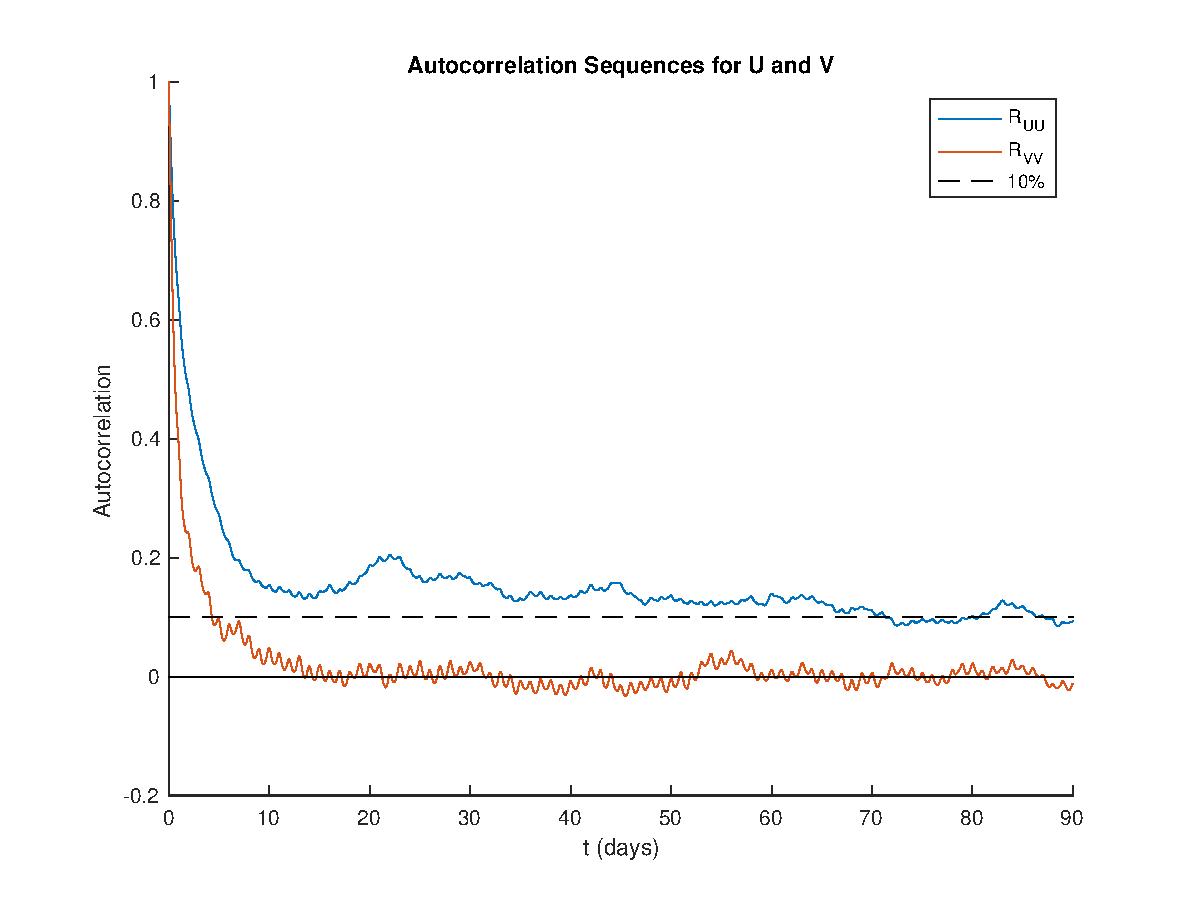
\includegraphics[width=\columnwidth]{figures/AutocorrelationSequences_90days}
\caption{Autocorrelation sequences $R_{UU}$ and $R_{VV}$.}
\label{fig:Autocorrelations}
\end{figure}

According to these values, we see that the stream-wise winds tend to remain correlated for $\sim 5.5$ days, while the cross-stream winds remain correlated for only $\sim 2$ days.
Consequently, we can expect the errors incurred by the autoregression method to reach a relatively constant value after $\sim 5.5$ days.
Similarly, we can expect the errors generated by the persistence model to reach match those of the random sample method after $\sim 5.5$ days.

\subsection{Performance Characterization}
Here, we construct an autoregressive model, as described in \secref{sec:Methods:Autoregression}, with an order $P$ corresponding to 2 days, i.e., $P = 2 \times 24 F_s$, where $F_s$ is given in samples per hour.
In each analysis below, we have computed, using \eqnref{eq:RMSError}, the rms error averaged over $Q = 100$ test segments.

\subsubsection{Comparison of Forecasting Methods}\label{sec:Results:Comparison}
The rms prediction errors incurred by each forecasting method are plotted in \figref{fig:ComparisonRMS}.
Here, we take $N_\text{in}$ and $N_\text{out}$ to correspond to 10 and 30 days, respectively.
%%TODO%% redo with N_in = 2 days
From this plot, we see that the autoregression method performs consistently superior to both the persistence and random sample methods.

\begin{figure}[htb]
\centering
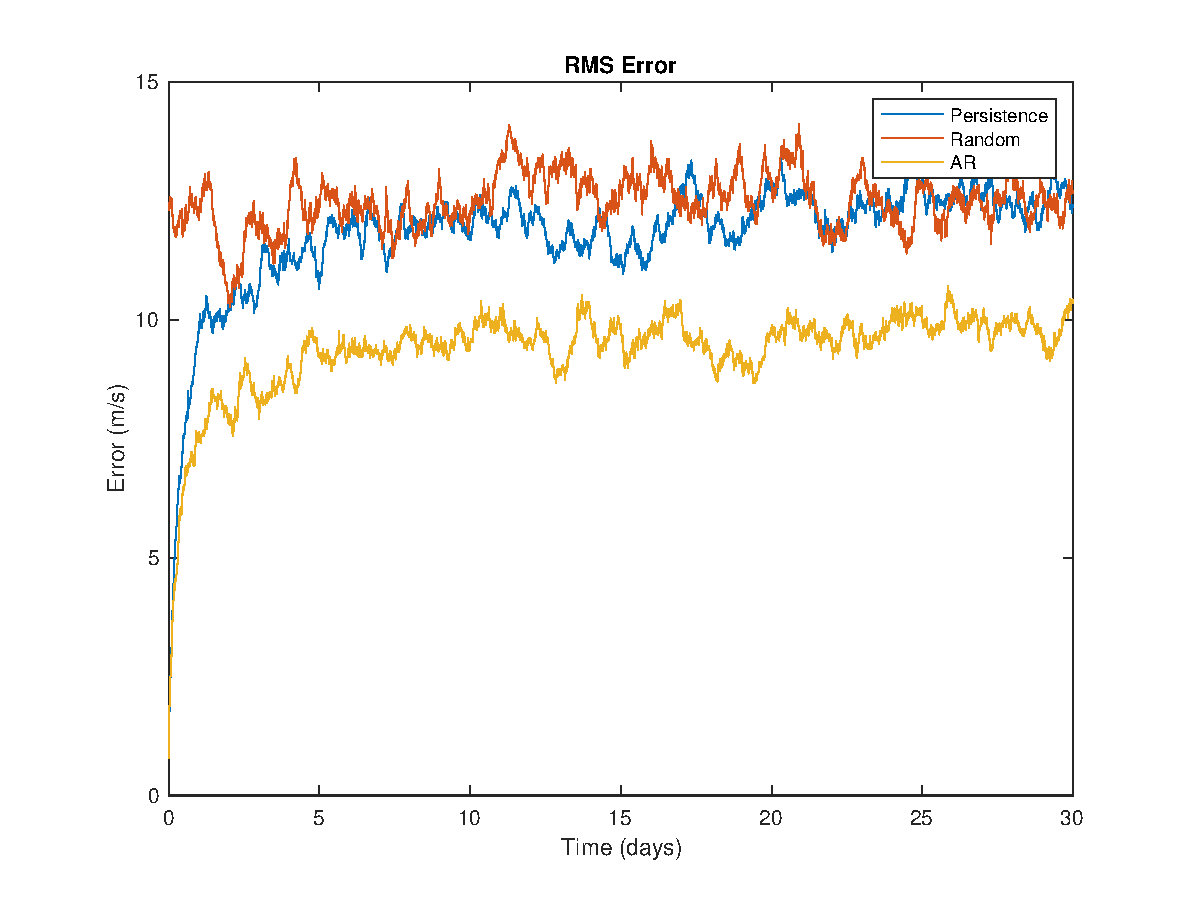
\includegraphics[width=\columnwidth]{figures/ComparisonRMSPredictionError}
\caption{Comparison of rms prediction errors.}
\label{fig:ComparisonRMS}
\end{figure}

For the random sample method, we would expect that the randomly selected ``predicted'' wind velocities will generally be uncorrelated with the reference wind velocities.
Accordingly, from \figref{fig:ComparisonRMS}, we see that the rms errors incurred by the random sample method are relatively constant with $n$.
However, for the persistence method, we see that the rms errors are small at small $t_n$, but ultimately reach similar values to those incurred by the random sample method.
We interpret this behavior as corresponding to the system ``forgetting'' about the previous wind conditions, and, in particular, we see that this happens when $t_n \approx T_U \approx 5.5$ days.

Similarly, we see that the autoregression method reaches a similar plateau in rms error beyond $T_U$.
However, these errors are still smaller than those of the persistence and random sample methods.
This suggests that, even though the system has ``forgotten'' about the previous wind conditions, the autoregression model is able to achieve predictions that are \textit{slightly} more accurate than the totally independent predictions produced by the alternative methods.

\subsubsection{Seasonal and Diurnal Performance}
The rms prediction errors incurred by the autoregression method are plotted for each season in \figref{fig:SeasonalRMS}.
From this plot, we see that the errors are smallest in the Summer and largest in the Winter.
This might suggest that wind conditions in the Spring or Summer tend to be ``more predictable'' than those in the Fall or Winter.

\begin{figure}[htb]
\centering
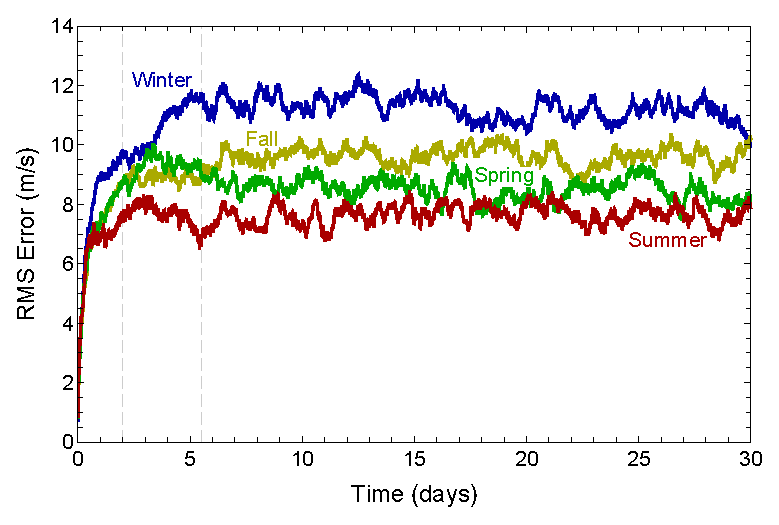
\includegraphics[width=\columnwidth]{figures/SeasonalRMSPredictionError}
\caption{Seasonal dependence of rms prediction errors.}
\label{fig:SeasonalRMS}
\end{figure}

The rms prediction errors incurred by the autoregression method under daytime and nighttime conditions are plotted in \figref{fig:DiurnalRMS}.
From this plot, we see that the prediction errors incurred during the daytime are consistently smaller than those incurred at night.
This is somewhat surprising, as we might expect nighttime conditions to be ``more predictable'' due to the stability of the atmospheric boundary layer.
However, what these results suggest is that the autoregression method is better able to predict daytime wind conditions given data from the previous night, than it is to predict nighttime wind conditions given data from the previous day.
Consequently, we infer that nighttime wind conditions are more useful predictors of the following day's wind conditions than the opposite.

\begin{figure}[htb]
\centering
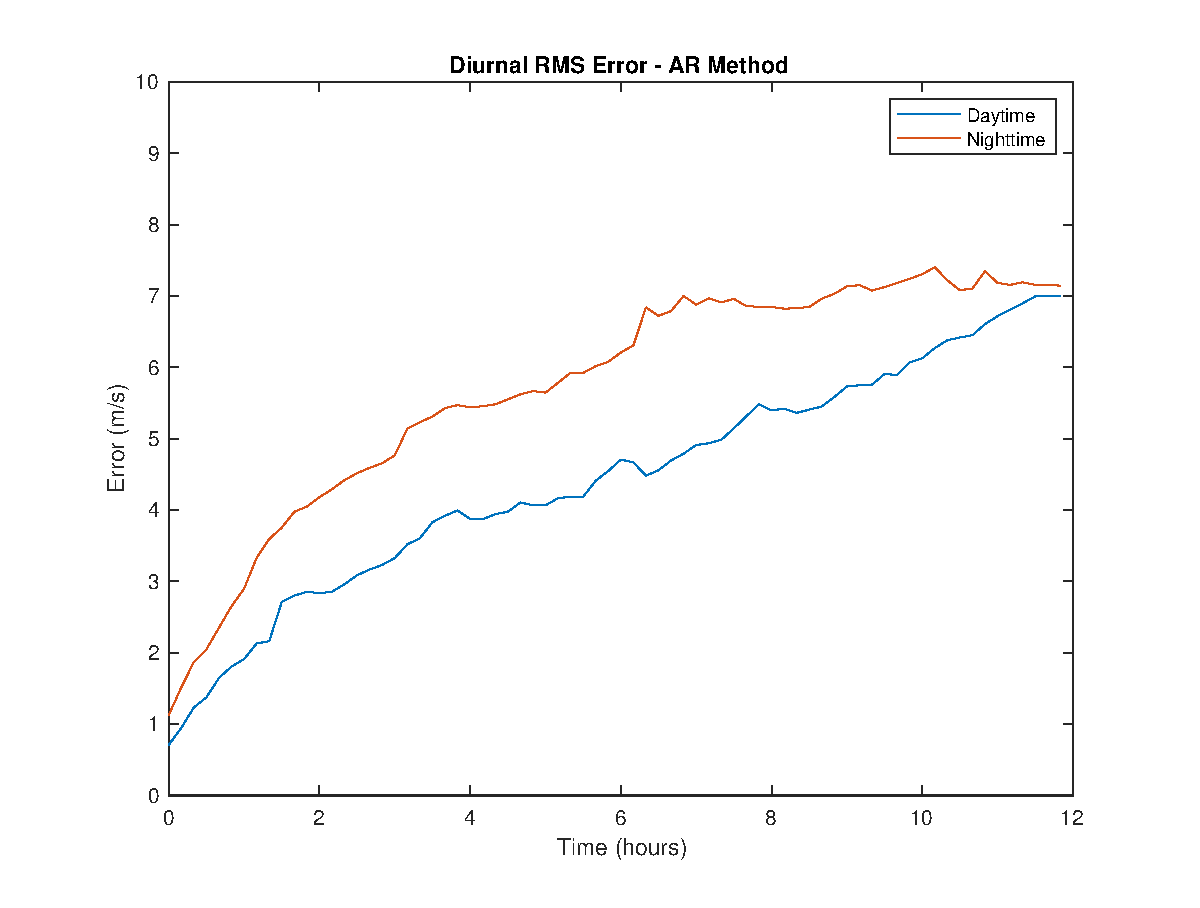
\includegraphics[width=\columnwidth]{figures/DiurnalRMSPredictionError}
\caption{Diurnal dependence of rms prediction errors.}
\label{fig:DiurnalRMS}
\end{figure}

%%%% CONCLUSIONS %%%%
\section{Summary and Conclusions}\label{sec:Conclusions}
In this work we implemented and characterized the performance of an autoregression model for wind velocity forecasting.
We first determined the relevant timescales over which an autoregression model can be expected to perform well by conducting an autocorrelation analysis using a dataset of historical wind data.
Subsequently, we compared, in terms of an average prediction error, the performance of the autoregression model to that of two simpler predictive models: a persistence model and a random sample.
Additionally, we examined the variation of prediction error with season and under daytime and nighttime conditions.

Results of the timescale analysis suggest that the wind system will tend to ``forget'' previous wind conditions after approximately 5.5 days (see \secref{sec:Results:Timescale}).
Indeed, results show that, while the autoregression model performs consistently superior to the simpler alternative models, it reaches a plateau in prediction error over approximately that timescale (see \figref{fig:ComparisonRMS}).
The autoregression model was also found to yield more accurate predictions in the Summer than in the Winter (see \figref{fig:SeasonalRMS}), which suggests that wind conditions in the Summer may be more consistent and ``predictable'' as a result.
Daytime predictions of wind velocity were also found to be more accurate than nighttime predictions (see \figref{fig:DiurnalRMS}), which suggests that nighttime wind conditions are more useful predictors of the following day's wind conditions than the opposite.

\subsection{Future Work}
Future investigations should include an implementation of more specific or localized autoregression models.
For example, different autoregression coefficients might be computed for each season and/or for each time of day.

\bibliographystyle{unsrtnat}
\bibliography{refs}

\end{document}